\section{The geometric obstruction}
\label{sec:obstruction}

We now show that the configuration obtained in
Proposition~\ref{prop:configuration} cannot occur in a complete $\CAT(0)$
space.  The argument takes place first in that space and then in its
completed tangent cone at the common hexagon center.  The tangent cone
is not assumed to be a vector space, so we specify the meaning of its
sums and use concavity whenever an additive inequality is required.

\subsection{Cone notation and square rigidity}

For a $\CAT(0)$ Euclidean cone $T$ with vertex $0$, let $\delta_a$ denote
radial dilation by $a\geq 0$.  Write $a u=\delta_a(u)$ and
\[
 \norm{u}=d_T(0,u),\qquad
 \ip{u}{v}=\frac{\norm{u}^2+\norm{v}^2-d_T(u,v)^2}{2}.
\]
For nonzero vectors this last expression is
$\norm{u}\norm{v}\cos\angle(u,v)$, where the angular distance is
truncated at $\pi$.  Define
\begin{equation}
 u\oplus v=2\operatorname{mid}(u,v).
 \label{geom:cone-addition}
\end{equation}
This operation is commutative, but no associativity or cancellation law
will be used.  If the directions of $u,v$ are joined by a geodesic of
length less than $\pi$, its cone is a Euclidean sector, and
$u\oplus v$ is the ordinary vector sum in that sector.  More generally,
all two-vector calculations below are either made in such a sector or
follow from the metric definition in Equation~\eqref{geom:cone-addition}.

The scalar-product concavity established in Lemma~\ref{energy:cone-mean}
implies
\begin{equation}
 \ip{w}{u\oplus v}\geq \ip{w}{u}+\ip{w}{v}.
 \label{geom:sum-concavity}
\end{equation}
Indeed, apply concavity at the midpoint of $u,v$ and use homogeneity
under radial dilation.  This is an inequality in a general cone; we
will not replace it by an equality without establishing rigidity.

We use two established equality principles for $\CAT(0)$ spaces.  A
triangle is flat if one vertex angle equals its Euclidean comparison
angle, or if a nontrivial interior comparison inequality is an
equality; see \cite[Proposition~II.2.9 and
Exercise~II.2.10(1)]{BH1999} and
\cite[Proposition~I.3.13(ii)]{Ballmann1995}.  Here and below, flat means that the
convex hull is isometric to the corresponding Euclidean triangle.

\begin{lemma}[Square rigidity]
\label{geom:square}
Let $p_0,p_1,p_2,p_3$ be points of a $\CAT(0)$ space, with indices
taken modulo four.  Suppose
\[
 d(p_i,p_{i+1})=1,\qquad
 d(p_0,p_2)=d(p_1,p_3)=\sqrt{2}.
\]
Their convex hull is a unit Euclidean square, in the indicated cyclic
order.  In particular, the two diagonals have the same midpoint.
\end{lemma}

\begin{proof}
Let $o$ be the midpoint of $p_0,p_2$.  Squared-distance convexity gives
\[
 d(o,p_1)^2\leq\frac12,\qquad d(o,p_3)^2\leq\frac12.
\]
Since
\[
 \sqrt2=d(p_1,p_3)\leq d(p_1,o)+d(o,p_3)\leq\sqrt2,
\]
both inequalities are equalities and $o$ is also the midpoint of
$p_1,p_3$.  The equality for $d(o,p_1)$ is an interior comparison
equality in the triangle $p_1,p_0,p_2$, so that triangle is flat.  The
same argument, with each of the four vertices as the vertex opposite
a diagonal midpoint, makes each triangle on three consecutive vertices
flat.  The angle at each corner of the quadrilateral is therefore
$\pi/2$.  The flat quadrilateral theorem
\cite[Theorem~II.2.11]{BH1999} applies: the sum of these four angles is
$2\pi$.  Its Euclidean quadrilateral has the prescribed sides and
diagonals, and hence is a unit square.
\end{proof}

\subsection{The sums at the four doubled points}

Suppose that $Z$ is a complete $\CAT(0)$ space containing the
configuration from Proposition~\ref{prop:configuration}.  Use the graph
vertex names for the corresponding points of $Z$.  Let $c$ be the common
hexagon center and put
\[
 r=\frac{\sqrt3}{2},\qquad T=T_c Z.
\]
The completed tangent cone $T$ is $\CAT(0)$, and its completed space of
directions is $\CAT(1)$ by \cite[Theorem~II.3.19]{BH1999}.  Write
\[
 x_i=\log_c X_i,\qquad y_i=\log_c Y_i,\qquad
 h_H=\log_c H
\]
for the named radial vectors, and abbreviate $h_{ij}=h_H$ when
$H=ij$.  All these vectors have norm $r$.

Any two distinct line vertices $H,H'$ occur together in a core
hexagon: take their intersection point $i$, choose a point $j\ne i$
on $H$ and a point $k\ne i$ on $H'$, and use the $X$ representatives
of the noncollinear triple $i,j,k$.  Their central triangle is flat
by Proposition~\ref{prop:configuration}, and their distance is
$\sqrt2$.  Consequently
\begin{equation}
 \ip{h_H}{h_{H'}}=-\frac14
 \quad\text{for distinct lines }H,H'.
 \label{geom:line-products}
\end{equation}

A line through a doubled point $i\in\{A,B,C,D\}$ is called
\emph{full at $i$} if it is adjacent to both $X_i$ and $Y_i$.
All lines through $A,B,C$ are full; the full lines at $D$ are $AD,BD$.

\begin{lemma}[Fan identities]
\label{geom:fan-sums}
For $i\in\{A,B,C,D\}$ there is a unit vector $M_i\in T$ such that
\begin{equation}
 M_i=x_i\oplus y_i=h_H\oplus h_{H'}
 \quad\text{whenever }H,H'\text{ are distinct full lines at }i.
 \label{geom:fan-identities}
\end{equation}
Each sum displayed here is computed in a nondegenerate Euclidean
sector.  Moreover,
\begin{equation}
 \ip{x_i}{y_i}=-\frac14,
 \qquad
 \ip{M_i}{h_H}=\ip{M_i}{h_{H'}}=\frac12.
 \label{geom:fan-products}
\end{equation}
\end{lemma}

\begin{proof}
The four-cycle $X_i,H,Y_i,H'$ has unit sides and diagonals of length
$\sqrt2$, by the two-step assertions of
Proposition~\ref{prop:configuration}.  Lemma~\ref{geom:square} makes it
a flat square.  Let $J_i$ be its center, which is the midpoint of
$X_i,Y_i$ and also of $H,H'$.

The triangle $c,H,H'$ is flat.  Its median therefore gives
\[
 d(c,J_i)^2=r^2-\frac14 d(H,H')^2=\frac14.
\]
On the other hand, squared-distance convexity in the triangle
$c,X_i,Y_i$ has right-hand side
\[
 \frac12 d(c,X_i)^2+\frac12 d(c,Y_i)^2
       -\frac14 d(X_i,Y_i)^2
 =\frac14.
\]
Thus this is also an equality, and $c,X_i,Y_i$ is a flat triangle.
Taking its midpoint in the tangent cone proves
\[
 x_i\oplus y_i=2\log_c J_i=h_H\oplus h_{H'}.
\]
Define $M_i=2\log_c J_i$; it has norm one.  The left-hand side makes
it independent of the full-line pair chosen.  The cosine law gives
$\ip{x_i}{y_i}=-1/4$.  The pair $h_H,h_{H'}$ has angular separation
$\arccos(-1/3)<\pi$, and in its Euclidean sector
\[
 \ip{h_H\oplus h_{H'}}{h_H}
 =\norm{h_H}^2+\ip{h_{H'}}{h_H}
 =\frac34-\frac14=\frac12.
\]
The same computation applies to $h_{H'}$.
\end{proof}

We will obtain a contradiction by evaluating the scalar product of
the unit vectors $M_A,M_B$ in two ways.  One bound is already
available.  At $A,B$, the fan identities give
\[
 M_A=h_{AB}\oplus h_{AC},\qquad
 M_B=h_{AB}\oplus h_{BC}.
\]
Apply Equation~\eqref{geom:sum-concavity} in both entries.  The three
lines $AB,AC,BC$ are distinct, so
Equation~\eqref{geom:line-products} yields
\begin{equation}
 \ip{M_A}{M_B}
 \geq\norm{h_{AB}}^2+\ip{h_{AB}}{h_{BC}}
       +\ip{h_{AC}}{h_{AB}}+\ip{h_{AC}}{h_{BC}}
 =0.
 \label{geom:nonnegative}
\end{equation}
The remaining argument will force $M_A,M_B$ to be antipodal, with
scalar product $-1$.  We first use the exceptional incidence to show
that $M_C,M_D$ are antipodal.  Their axis will let us place
$h_{AC},h_{BC},h_{AD},h_{BD}$ in a product $\mathbb R\times Q$,
where the $\CAT(0)$ factor $Q$ contains a flat square formed by
their second coordinates.  The opposite side midpoints of that square
will then force $M_A,M_B$ to be antipodal through the fan identities
at $A,B$.

\subsection{The identity at the exceptional incidence}

Set
\[
 H_0=CD,\qquad h_0=h_{CD},\qquad
 p=X_C,\quad q=Y_C,\quad z=X_D,
\]
and let $J$ be the midpoint of $p,q$.  The missing edge from $Y_D$
to $H_0$ is responsible for the asymmetry used in the next lemma.

\begin{lemma}[Exceptional-incidence identity]
\label{geom:exceptional}
The vectors $M_C,x_D$ lie in a Euclidean sector in $T$, and
\begin{equation}
 h_0=M_C\oplus x_D.
 \label{geom:exceptional-sum}
\end{equation}
Within this sector,
\begin{equation}
 \ip{M_C}{x_D}=-\frac12,\qquad
 \ip{M_C}{h_0}=\frac12,\qquad
 \ip{h_0}{x_D}=\frac14.
 \label{geom:exceptional-products}
\end{equation}
\end{lemma}

\begin{proof}
Apply the square construction in Lemma~\ref{geom:fan-sums} at $C$,
using $H_0$ and any other line through $C$.  Since $J$ is its center,
\begin{equation}
 d(H_0,J)^2=\frac12,\qquad d(c,J)^2=\frac14.
 \label{geom:exceptional-distances}
\end{equation}
Also $d(H_0,z)=1$, $d(c,z)=d(c,H_0)=r$, and the two paths
$p,H_0,z$ and $q,H_0,z$ give
\[
 d(p,z)^2=d(q,z)^2=2.
\]
The ternary midpoint conclusion of
Proposition~\ref{prop:configuration} states that the angle at $H_0$
between the segments to $J,z$ is at least $\pi/2$.  Angle comparison
and Equation~\eqref{geom:exceptional-distances} therefore imply
\[
 d(J,z)^2\geq d(H_0,J)^2+d(H_0,z)^2=\frac32.
\]
The reverse inequality follows from the fact that $J$ is the midpoint
of $p,q$:
\[
 d(J,z)^2\leq\frac12d(p,z)^2+\frac12d(q,z)^2
                    -\frac14d(p,q)^2=\frac32.
\]
The angle and distance comparisons are consequently equalities.
The triangle $H_0,J,z$ is flat, with a right angle at $H_0$.

Let $B_0$ be the point of $[J,z]$ at parameter $1/3$ from $J$.
Calculating in this right triangle gives
\[
 d(H_0,B_0)^2
 =\left(\frac23\right)^2\frac12
  +\left(\frac13\right)^2=\frac13.
\]
Squared-distance convexity toward $c$ gives
\begin{align*}
 d(c,B_0)^2
 &\leq\frac23 d(c,J)^2+\frac13d(c,z)^2
                 -\frac29d(J,z)^2\\
 &=\frac23\frac14+\frac13\frac34-\frac29\frac32
 =\frac1{12}.
\end{align*}
The triangle inequality now reads
\[
 \frac{\sqrt3}{2}=d(H_0,c)
 \leq d(H_0,B_0)+d(B_0,c)
 \leq\frac1{\sqrt3}+\frac1{2\sqrt3}
 =\frac{\sqrt3}{2}.
\]
Hence every inequality is an equality.  In particular, $B_0$ lies on
$[H_0,c]$, in that order, and the triangle $c,J,z$ is flat by its
interior comparison equality.  Put $j=\log_c J$.  In the Euclidean
sector containing $j,x_D$, the vector to $B_0$ is
$(2/3)j+(1/3)x_D$.  The collinearity just proved and the distances
$d(c,H_0)=3d(c,B_0)$ therefore imply
\[
 h_0=3\log_c B_0=2j+x_D=M_C\oplus x_D.
\]
Here the two ordinary additions take place in that Euclidean sector,
and $M_C=2j$ by Lemma~\ref{geom:fan-sums}.

The norm identity in this sector gives
\[
 \frac34=\norm{h_0}^2
 =1+\frac34+2\ip{M_C}{x_D},
\]
so $\ip{M_C}{x_D}=-1/2$.  Pairing the sector identity with either
summand yields the remaining two products in
Equation~\eqref{geom:exceptional-products}.
\end{proof}

\subsection{A semicircle in the space of directions}

\begin{lemma}
\label{geom:antipodal}
The unit vectors $M_C,M_D$ are antipodal in $T$:
\[
 d_T(M_C,M_D)=2,\qquad \ip{M_C}{M_D}=-1.
\]
\end{lemma}

\begin{proof}
Take either full line $H$ at $D$.  The path
$Y_D,H,X_D,H_0$ uses two fields of $F_D$ and the loose field, so it is
one of the admissible three-step paths.  Thus
\[
 d(Y_D,H_0)\geq\sqrt3=d(Y_D,c)+d(c,H_0).
\]
Equality follows from the triangle inequality.  The segment from
$Y_D$ to $H_0$ passes through $c$, and the directions of $y_D,h_0$
are antipodal.

Let $\Sigma$ be the completed space of directions of $Z$ at $c$, and
use a hat for the direction of a nonzero vector.  Define
\[
 a=\arccos(1/\sqrt3),\qquad b=\arccos(1/3).
\]
Both lie strictly between zero and $\pi/2$, and $2a+b=\pi$.
Equation~\eqref{geom:exceptional-products} gives
\[
 d_\Sigma(\widehat M_C,\widehat h_0)=a,
 \qquad d_\Sigma(\widehat h_0,\widehat x_D)=b.
\]
The two arcs occur consecutively in the Euclidean sector of
Lemma~\ref{geom:exceptional}; their concatenation is its geodesic
direction arc.  By Equation~\eqref{geom:fan-products},
\[
 d_\Sigma(\widehat x_D,\widehat y_D)=\arccos(-1/3)=\pi-b.
\]
The direction of $M_D=x_D\oplus y_D$ bisects this last arc, because
its two summands have equal length.  Consequently
$d_\Sigma(\widehat x_D,\widehat M_D)=a$.

The concatenation
$\widehat h_0,\widehat x_D,\widehat y_D$ has length $\pi$ and
antipodal endpoints.  It is therefore minimizing, so its two arcs
continue geodesically through $\widehat x_D$.  It follows that
\[
 \widehat M_C,\quad\widehat h_0,\quad\widehat x_D,
 \quad\widehat M_D
\]
is a local geodesic in $\Sigma$: continuation at $\widehat h_0$
holds inside the first sector, and continuation at $\widehat x_D$
holds inside the minimizing semicircle just described.  Its length
is $a+b+a=\pi$.  The space $\Sigma$ is $\CAT(1)$, so
\cite[Proposition~II.1.4(2)]{BH1999} makes this local geodesic
globally minimizing, including the endpoint case of length exactly
$\pi$.  Equivalently, apply the short local-geodesic assertion to
every strict initial subarc and pass to the endpoint by continuity
of distance.  Its endpoints are antipodal.  Since $M_C,M_D$ have norm
one, the cone distance and scalar product have the stated values.
\end{proof}

\subsection{Splitting the axis and obtaining a flat square}

\begin{proposition}
\label{prop:no-configuration}
No complete $\CAT(0)$ space contains the configuration asserted in
Proposition~\ref{prop:configuration}.
\end{proposition}

\begin{proof}
Suppose otherwise and retain the notation above.  By
Equation~\eqref{geom:nonnegative}, $\ip{M_A}{M_B}\geq0$.
We will contradict this bound by splitting the axis supplied by
Lemma~\ref{geom:antipodal}.  Use the fan identities
\[
 M_C=h_{AC}\oplus h_{BC},\qquad
 M_D=h_{AD}\oplus h_{BD}.
\]
The four lines in these expressions are pairwise distinct.  Therefore
Equation~\eqref{geom:sum-concavity} implies
\[
 \ip{M_C}{h_{AD}}\geq-\frac12,
 \qquad \ip{M_C}{h_{BD}}\geq-\frac12.
\]
Lemma~\ref{geom:antipodal} forces equality in the chain
\[
 -1=\ip{M_C}{M_D}
 \geq\ip{M_C}{h_{AD}}+\ip{M_C}{h_{BD}}\geq-1.
\]
Interchanging the roles of the two sums gives the symmetric
equalities.  Combining these with
Equation~\eqref{geom:fan-products}, we obtain
\begin{equation}
\begin{array}{c|rrrr}
 &h_{AC}&h_{BC}&h_{AD}&h_{BD}\\ \hline
 \ip{M_C}{\,\cdot\,}& 1/2&1/2&-1/2&-1/2\\
 \ip{M_D}{\,\cdot\,}&-1/2&-1/2& 1/2& 1/2.
\end{array}
\label{geom:axis-products}
\end{equation}

The opposite rays $M_C,M_D$ form a complete geodesic line
$\ell\subset T$ through the cone vertex.  Put
$a=\arccos(1/\sqrt3)$.  For each vector in the
four columns of Equation~\eqref{geom:axis-products}, the angles to
the two ends of $\ell$ are $a$ and $\pi-a$, in one order or the
other.  The two corresponding direction arcs concatenate to a
minimizing semicircle.  Its Euclidean cone is an isometric flat
half-plane with boundary $\ell$ and containing the vector.  In
particular, that vector lies on a complete line parallel to $\ell$.

The parallel-set product decomposition
\cite[Theorem~II.2.14]{BH1999} now applies in $T$; it requires no
properness.  Write its convex parallel set as
\[
 P(\ell)=\R\times Q,\qquad
 \ell=\R\times\{q_0\},\qquad
 0=(0,q_0),\quad M_C=(1,q_0),\quad M_D=(-1,q_0).
\]
The factor $Q$ is a $\CAT(0)$ space.  Within each of the flat
half-planes above, projection onto $\ell$ shows that the axial
coordinate is the scalar product with the unit vector $M_C$.
Thus Equation~\eqref{geom:axis-products} gives
\begin{equation}
 h_{AC}=(1/2,u),\quad h_{BC}=(1/2,u'),\quad
 h_{AD}=(-1/2,v),\quad h_{BD}=(-1/2,v')
 \label{geom:split-coordinates}
\end{equation}
for points $u,u',v,v'\in Q$.  Their distances to $q_0$ are all
$1/\sqrt2$, since each original vector has squared norm $3/4$.

Distinct line vectors have squared cone distance two, by
Equation~\eqref{geom:line-products}.  The product metric in
Equation~\eqref{geom:split-coordinates} therefore gives
\[
 d_Q(u,u')=d_Q(v,v')=\sqrt2,
\]
and
\[
 d_Q(u,v)=d_Q(u,v')=d_Q(u',v)=d_Q(u',v')=1.
\]
Furthermore, $h_{AC}\oplus h_{BC}=M_C$ means that the midpoint
of these two line vectors is $(1/2,q_0)$: the midpoint is the
half-dilation of $M_C$ on the axis.  Product midpoints consequently
give $q_0=\operatorname{mid}(u,u')$.  The identity at $D$ likewise
gives $q_0=\operatorname{mid}(v,v')$.

In cyclic order $u,v,u',v'$, these points satisfy
Lemma~\ref{geom:square}.  They therefore span a unit flat square
in $Q$, centered at $q_0$.  Let
\[
 m=\operatorname{mid}(u,v),\qquad
 m'=\operatorname{mid}(u',v').
\]
They are the midpoints of opposite sides of that square, and hence
\begin{equation}
 d_Q(q_0,m)=d_Q(q_0,m')=\frac12,
 \qquad d_Q(m,m')=1.
 \label{geom:opposite-midpoints}
\end{equation}
This square lies in the transverse factor only; no planar realization
of the original incidence configuration has been assumed.
Figure~\ref{fig:transverse-square} records the square and the axis that
has been split off.

\begin{figure}[htbp]
\centering
\begin{minipage}[c]{.43\textwidth}
\centering
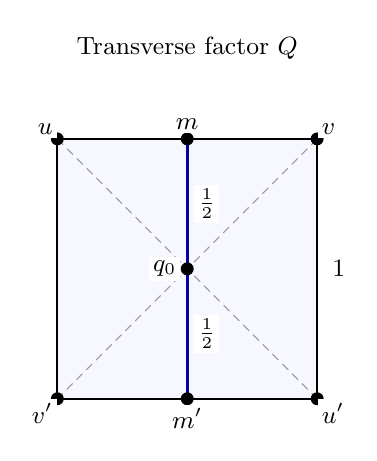
\begin{tikzpicture}[x=3.3cm,y=3.3cm,
  square vertex/.style={circle,fill=black,inner sep=1.65pt},
  square label/.style={font=\small,fill=white,inner sep=1.5pt}]
  \coordinate (u) at (-.5,.5);
  \coordinate (v) at (.5,.5);
  \coordinate (up) at (.5,-.5);
  \coordinate (vp) at (-.5,-.5);
  \coordinate (m) at (0,.5);
  \coordinate (mp) at (0,-.5);
  \coordinate (q) at (0,0);
  \fill[blue!3] (u)--(v)--(up)--(vp)--cycle;
  \draw[draw=black!40,densely dashed] (u)--(up) (v)--(vp);
  \draw[line width=.85pt] (u)--(v)--(up)--(vp)--cycle;
  \draw[draw=blue!65!black,line width=1.2pt] (m)--(mp);
  \foreach \P in {u,v,up,vp,m,mp,q}
    \node[square vertex] at (\P) {};
  \node[square label,anchor=south east] at (u) {$u$};
  \node[square label,anchor=south west] at (v) {$v$};
  \node[square label,anchor=north west] at (up) {$u'$};
  \node[square label,anchor=north east] at (vp) {$v'$};
  \node[square label,anchor=south] at (0,.52) {$m$};
  \node[square label,anchor=north] at (0,-.52) {$m'$};
  \node[square label,anchor=east] at (-.025,0) {$q_0$};
  \node[square label,anchor=west] at (.025,.25) {$\frac12$};
  \node[square label,anchor=west] at (.025,-.25) {$\frac12$};
  \node[square label,anchor=west] at (.54,0) {$1$};
  \node[font=\small] at (0,.85) {Transverse factor $Q$};
\end{tikzpicture}
\end{minipage}\hfill
\begin{minipage}[c]{.53\textwidth}
\centering
\begin{tikzpicture}[x=2.05cm,y=1cm,
  axis label/.style={font=\small,fill=white,inner sep=1.5pt}]
  \draw[{Stealth[length=4pt]}-{Stealth[length=4pt]},line width=.7pt]
    (-1.22,0)--(1.22,0);
  \foreach \x in {-1,0,1}\fill (\x,0) circle[radius=1.65pt];
  \node[axis label,anchor=south] at (-1,.07) {$M_D$};
  \node[axis label,anchor=south] at (1,.07) {$M_C$};
  \node[axis label,anchor=north] at (0,-.07) {$0_T$};
  \node[font=\small] at (0,.9) {Axis $\ell=\mathbb R\times\{q_0\}$};
\end{tikzpicture}
\par\smallskip
$P(\ell)\cong\mathbb R\times Q$\par\medskip
$M_A=2(0,m),\qquad M_B=2(0,m')$
\end{minipage}
\caption{The final contradiction takes place in the transverse factor after
splitting off the $M_C,M_D$ axis.  The cyclically ordered points $u,v,u',v'$
form a flat unit square in $Q$, with common diagonal midpoint $q_0$.
The opposite-side midpoints $m,m'$ are distance $1/2$ from $q_0$ and distance
$1$ apart.  Dilation in the original tangent cone $T$ therefore makes
$M_A=2(0,m)$ and $M_B=2(0,m')$ antipodal unit vectors.  The panels display
the two distinct factors of the parallel set.}
\label{fig:transverse-square}
\end{figure}


Finally, the full-line choices $AC,AD$ at $A$ and $BC,BD$ at $B$
give
\[
 M_A=h_{AC}\oplus h_{AD}=\delta_2(0,m),\qquad
 M_B=h_{BC}\oplus h_{BD}=\delta_2(0,m').
\]
Here $\delta_2$ is dilation in the original cone $T$; no cone
structure on $Q$ is needed.  It doubles all distances.  By
Equation~\eqref{geom:opposite-midpoints},
\[
 \norm{M_A}=\norm{M_B}=1,\qquad d_T(M_A,M_B)=2,
\]
so $\ip{M_A}{M_B}=-1$.  This contradicts
Equation~\eqref{geom:nonnegative} and proves the proposition.
\end{proof}
